% This is ''sig-alternate.tex'' V1.9 April 2009
% This file should be compiled with V2.4 of ''sig-alternate.cls'' April 2009
%
% This example file demonstrates the use of the 'sig-alternate.cls'
% V2.4 LaTeX2e document class file. It is for those submitting
% articles to ACM Conference Proceedings WHO DO NOT WISH TO
% STRICTLY ADHERE TO THE SIGS (PUBS-BOARD-ENDORSED) STYLE.
% The 'sig-alternate.cls' file will produce a similar-looking,
% albeit, 'tighter' paper resulting in, invariably, fewer pages.
%
% ----------------------------------------------------------------------------------------------------------------
% This .tex file (and associated .cls V2.4) produces:
%       1) The Permission Statement
%       2) The Conference (location) Info information
%       3) The Copyright Line with ACM data
%       4) NO page numbers
%
% as against the acm_proc_article-sp.cls file which
% DOES NOT produce 1) thru' 3) above.
%
% Using 'sig-alternate.cls' you have control, however, from within
% the source .tex file, over both the CopyrightYear
% (defaulted to 200X) and the ACM Copyright Data
% (defaulted to X-XXXXX-XX-X/XX/XX).
% e.g.
% \CopyrightYear{2007} will cause 2007 to appear in the copyright line.
% \crdata{0-12345-67-8/90/12} will cause 0-12345-67-8/90/12 to appear in the copyright line.
%
% ---------------------------------------------------------------------------------------------------------------
% This .tex source is an example which *does* use
% the .bib file (from which the .bbl file % is produced).
% REMEMBER HOWEVER: After having produced the .bbl file,
% and prior to final submission, you *NEED* to 'insert'
% your .bbl file into your source .tex file so as to provide
% ONE 'self-contained' source file.
%
% ================= IF YOU HAVE QUESTIONS =======================
% Questions regarding the SIGS styles, SIGS policies and
% procedures, Conferences etc. should be sent to
% Adrienne Griscti (griscti@acm.org)
%
% Technical questions _only_ to
% Gerald Murray (murray@hq.acm.org)
% ===============================================================
%
% For tracking purposes - this is V1.9 - April 2009

\documentclass{sig-alternate}
%\documentclass{acm_proc_article-sp}

\usepackage{mathptmx}
\usepackage{latexsym}
\usepackage{textcomp}
\usepackage{mathcomp}
\usepackage{stmaryrd}
\usepackage{amssymb}

\usepackage[sort]{natbib}
\usepackage{booktabs}

%TODO: load haskell
\usepackage{listings} \lstloadlanguages{C++} % there are many
\usepackage[caption=false]{subfig}
\usepackage{color}
\usepackage{alltt}
%\usepackage{my-macros}

%graphics stuff
\usepackage{graphicx}
\graphicspath{{pics/}}

%borders around figures
%\usepackage{float}
%\floatstyle{boxed} 
%\restylefloat{figure}

\begin{document}
%
% --- Author Metadata here ---
%\conferenceinfo{IHI'12,} {January 28--30, 2012, Miami, Florida, USA.} 
%\CopyrightYear{2012} 
%\crdata{978-1-4503-0781-9/12/01} 
%\clubpenalty=10000 
%\widowpenalty = 10000
% --- End of Author Metadata ---

\title{Frabjous|| : A Declarative Framework for Agent-Based Modelling}
%\subtitle{[Extended Abstract]
%\titlenote{A full version of this paper is available as
%\textit{Author's Guide to Preparing ACM SIG Proceedings Using
%\LaTeX$2_\epsilon$\ and BibTeX} at
%\texttt{www.acm.org/eaddress.htm}}}
%
% You need the command \numberofauthors to handle the 'placement
% and alignment' of the authors beneath the title.
%
% For aesthetic reasons, we recommend 'three authors at a time'
% i.e. three 'name/affiliation blocks' be placed beneath the title.
%
% NOTE: You are NOT restricted in how many 'rows' of
% ''name/affiliations'' may appear. We just ask that you restrict
% the number of 'columns' to three.
%
% Because of the available 'opening page real-estate'
% we ask you to refrain from putting more than six authors
% (two rows with three columns) beneath the article title.
% More than six makes the first-page appear very cluttered indeed.
%
% Use the \alignauthor commands to handle the names
% and affiliations for an 'aesthetic maximum' of six authors.
% Add names, affiliations, addresses for
% the seventh etc. author(s) as the argument for the
% \additionalauthors command.
% These 'additional authors' will be output/set for you
% without further effort on your part as the last section in
% the body of your article BEFORE References or any Appendices.

\numberofauthors{3} %  in this sample file, there are a *total*
% of EIGHT authors. SIX appear on the 'first-page' (for formatting
% reasons) and the remaining two appear in the \additionalauthors section.
%
\author{
% You can go ahead and credit any number of authors here,
% e.g. one 'row of three' or two rows (consisting of one row of three
% and a second row of one, two or three).
%
% The command \alignauthor (no curly braces needed) should
% precede each author name, affiliation/snail-mail address and
% e-mail address. Additionally, tag each line of
% affiliation/address with \affaddr, and tag the
% e-mail address with \email.
%
% 1st. author
\alignauthor
%\emph{Author names removed for anonymous review}
Ivan Vendrov\\
      \affaddr{Dept. of Computer Science}\\
      \affaddr{University of Saskatchewan}\\
      \affaddr{Saskatoon, SK, Canada}\\
       \email{ivan.vendrov@usask.ca}
% 2nd. author
\alignauthor
Christopher Dutchyn\\
       \affaddr{Dept. of Computer Science}\\
       \affaddr{University of Saskatchewan}\\
       \affaddr{Saskatoon, SK, Canada}\\
       \email{dutchyn@cs.usask.ca}
% 3rd. author
\alignauthor
Nathaniel Osgood\\
       \affaddr{Dept. of Computer Science}\\
       \affaddr{University of Saskatchewan}\\
       \affaddr{Saskatoon, SK, Canada}\\
       \email{osgood@cs.usask.ca}
}

%\date{30 June 2011}

\maketitle

\begin{abstract}
-todo-
\end{abstract}

% A category with the (minimum) three required fields
\category{D.3.2}{Programming Languages}{Language Classifications - \it functional, parallel, data-flow}
\category{I.6.5}{Simulation and Modeling}{Model Development}; Modeling Methodologies
\category{J.3}{Life and Medical Sciences}{Health} 

%!!!
\terms{Languages, Experimentation}

\keywords
Functional reactive, functional programming, simulation, dynamic model, domain-specific language, agent-based simulation, agent-based modelling, data parallel programming

\

\section{Introduction}

%Modelling complex systems is important. 

%The choice of language is crucial in determining the range of models produced - a language narrows or widens the "explanatory universe" for a given behaviour. Crucial interplay between the range and the ease of specification - technically any behaviour can be simulated by differential equations, but the language of differential equations is eminently ill-suited for thinking about stateful processes (give example). 

For systems that evolve continuously in space and time, the language of differential equations (DE's) - honed by centuries of application to the physical sciences - has no substitute. Its syntax is extremely terse, and it has a precise mathematical semantics that permits sophisticated analysis. While differential equations are not a natural fit for modelling populations of individuals (these being essentially discrete), the System Dynamics community has used them with great success to model the dynamics of large populations \textit{(insert citations  / examples)}. 

  There are, however,  a number of processes that are difficult if not impossible to feasibly express with differential equations, such as those involving networks or a high degree of heterogeneity in the populations being modelled \cite{system_dyn_tradeoffs}. The need to model these processes is addressed by agent based modelling (ABM), a far more general approach to modelling populations, which involves specifying the behaviour of each individual in the population and allowing the global dynamics to emerge from the interaction of individuals. 
  
  With the added flexibility and power of agent-based modelling there come a number of costs. With existing tools and frameworks, agent-based models are significantly harder to create, extend, and understand; significantly more expensive to calibrate and run; and significantly harder to mathematically analyze relative to models based on systems of differential equations \cite{ab_vs_de}. 
  
  Although the increased cognitive and computational costs of agent-based models are to some degree unavoidable due to the models' increased complexity and generality, we argue that these costs have been exacerbated by the use, in many ABM frameworks, of imperative languages like Java and C++. While these languages are well-suited for general-purpose programming, they are not good specification languages, due to their verbose nature and hiding of essential details. They generally force modellers and users to think at a lower level of abstraction, and fail to cleanly separate the relationships at the heart of the model from implementation details such as input/output, the time-stepping mechanism, and the data structures used \cite{system_dyn_tradeoffs}.
  
  On the other hand, the underlying language of DE models is not imperative but declarative - rather than explicitly specifying rules by which model variables change, differential equations specify relationships between model variables that hold at all times. We believe that the declarative nature of DE models accounts for much of their success by simplifying model creation, modification, and analysis. It then stands to reason that ABM could be similarly simplified by basing it on an appropriate declarative language. To support this hypothesis, we develop such a language and use it to implement a number of standard models from the literature. 
  
  \textit{possibly add more details about our contribution}.
  
\section{Background}
In this section, we briefly describe the existing languages and technologies, largely developed by the functional programming community, that we used to create Frabjous||.
\subsection{Haskell}

  Haskell is a purely functional language; that is to say, a Haskell program is a set of equations defining values and functions. (as close as we've gotten to the declarative ideal)


  
  
  
  
   




While computational health models have proven valuable lenses for understanding public health issues, such models are only now beginning to be applied to many pressing public health issues \cite{system_dyn_tradeoffs, system_dyn_approaches}. This in part reflects limits in the software support for modeling; the development of these models can be cumbersome, slow, and error-prone. %({cite-Nate})

The application of dynamic models to public health is further limited because such models are frequently challenging to build, difficult to understand and evaluate, computationally expensive, and difficult to share and collaboratively explore in policy decision teams.

A key aspect of this problem lies in how the models are specified and developed. Many are represented by imperative programming languages such as Java and Objective-C \cite{system_dyn_tradeoffs}. Despite the use of frameworks and problem-solving environments to handle the complexity of the code, these representations are fundamentally opaque and verbose. Developers must understand the programming language, the framework, and the model, which frequently demands considerable skills in software engineering.

Functional programming (FP), on the other hand, is well-doc\-u\-mented for being concise and transparent \cite{von_neumann,why_fp}. Also, functional languages are frequently easier to parallelize \cite{dphaskell, harness}. For an agent-based model with hundreds or thousands of agents working in parallel, parallel computing can greatly reduce the delay between scenario specification and the availability of results, facilitating experimentation and domain insight.

Although functional programming appears well-suited to representing simulation models, FP presents special difficulties for representing a time-varying system, since a functional style avoids a direct, mutable representation of the system state. As an alternative, we adopt functional reactive programming (FRP), originally developed by Elliot and Hudak \cite{fran}, to represent time as an intrinsic part of the paradigm.

In this work, we provide two main contributions. First, we explore a promising method for specifying agent-based epidemiological models with functional reactive programming by translating several models into Haskell/Yampa, an FRP framework. Second, we specify a domain-specific language, Frabjous, that generates readable and concise Haskell/Yampa code. Model specifications can be written, modified, or extended in either the Frabjous language or directly in Haskell/Yampa, leading to a flexible system that is transparent with respect to model structure and parameters.

We begin with a description of agent-based epidemiological simulation, and an overview of FRP. We then show how a simple model can be represented in FRP. We next give an overview for the Frabjous language and system. We conclude with our overall findings and future directions for this work.

%%%%%%%%%%%%%%
%	Section: Models	%
%%%%%%%%%%%%%%

\section{Computational Health Models}

In this section, we provide a brief overview of computational health models, current tools, and challenges encountered by modelers.

\subsection{The SIR Model}

One example of an agent-based health model is the classic \emph{Susceptible}, \emph{Infectious}, \emph{Recovered} (SIR) model (see Figure \ref{fig:sir}), which presents a stylized abstraction of the dynamics of infectious diseases such as measles, chickenpox, and pertussis \cite{AZPH:AZPH56}. Every agent in this system has one of three states - Susceptible, where the agent is not protected from the disease and may be infected; Infectious, where the agent is infected with the disease and may pass it on to Susceptible agents; and Recovered, where the agent no longer has the disease (and is temporarily or permanently protected from being infected). A simple version of this model has agents positioned on a two-dimensional grid, where each Susceptible neighbour of an Infectious agent has a defined probability of being infected. We will use this model as an example to illustrate our process and findings.

%if at all possible, I want have this on the front page for memorability
\begin{figure}[h]
%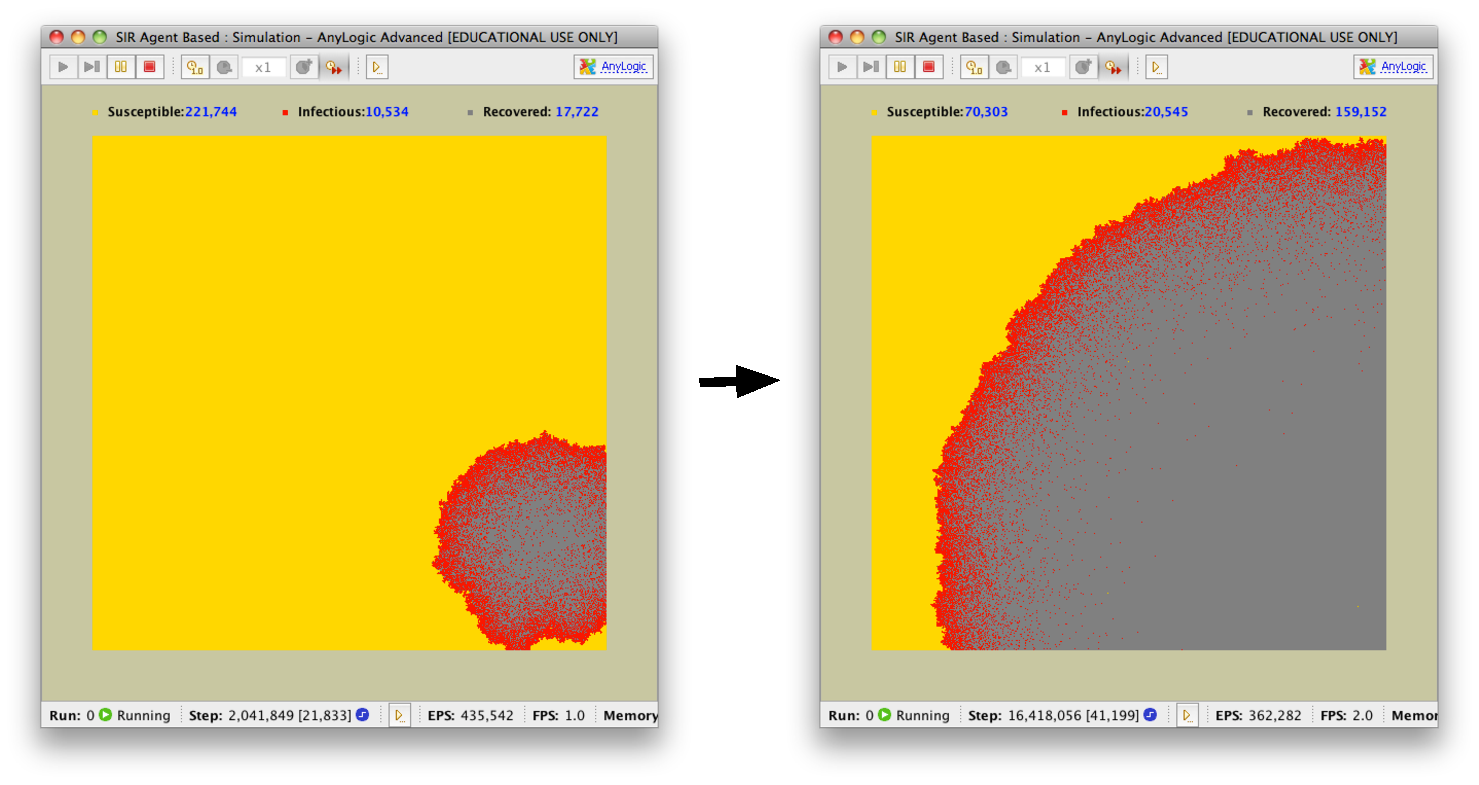
\includegraphics[ bb = 0 0 740 393, width=0.5\textwidth]{sir.pdf}
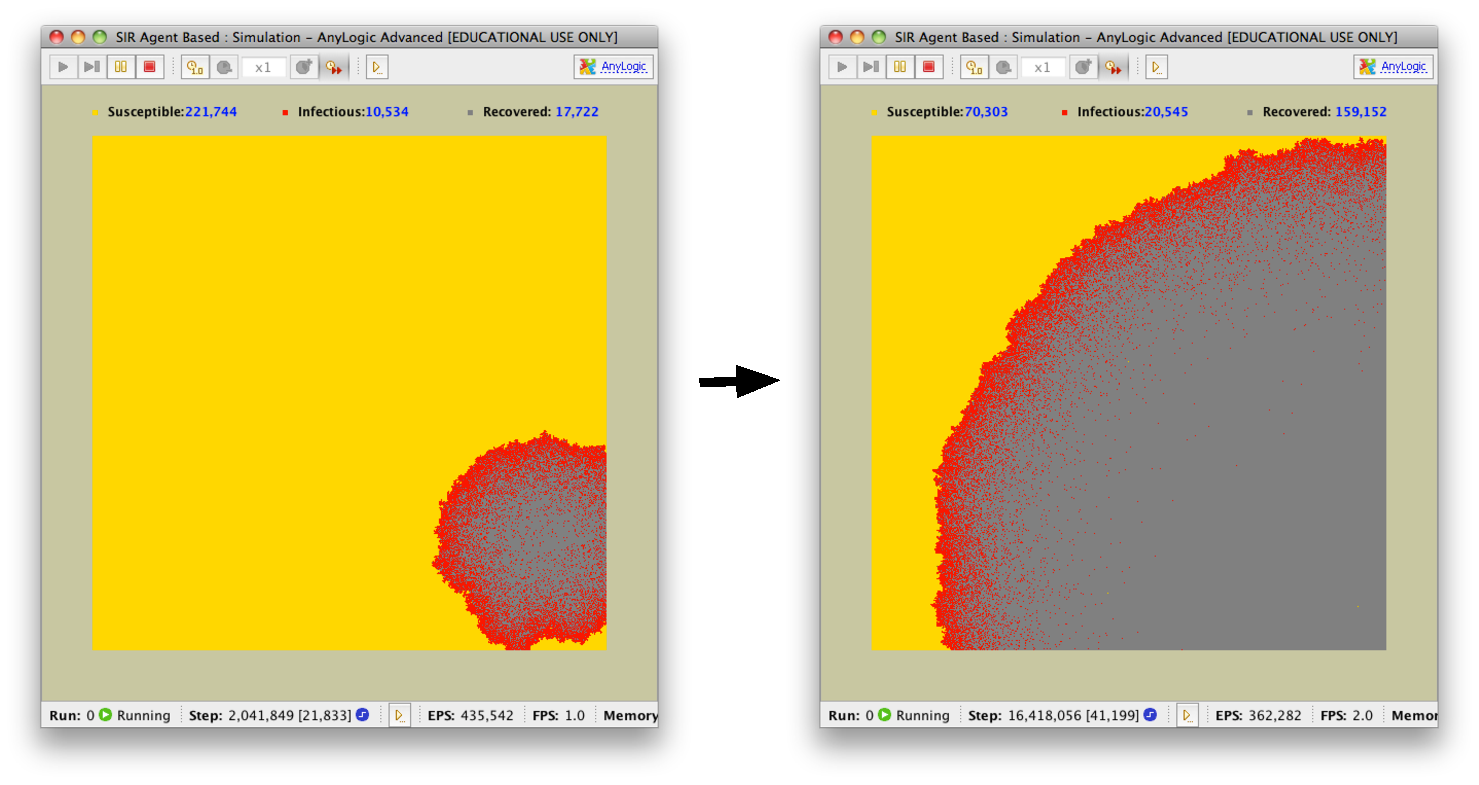
\includegraphics[width=0.5\textwidth]{sir.pdf}
\caption{SIR Model. Yellow squares are Susceptible agents, Red are Infectious, and Grey are Recovered. \label{fig:sir}}
\end{figure}

\subsection{Current Tools}
The past two decades have seen a rapid rise in the number of modeling packages supporting agent-based modeling.  These include REPAST/Simbuilder, SWARM, SDML, NETLOGO, and, most recently, AnyLogic \cite{North:2006:ECT:1122012.1122013, North2005, RePEc:wop:safiwp:96-06-042, Tisue04netlogo:design, springerlink:10.1023/A:1009600530279, anylogic}.

Most of these systems require custom programming to fine-tune simulation behaviour and analyze model operation.  Traditionally, agent-based models have been created in imperative programming languages such as Java and Objective-C \cite{system_dyn_approaches, system_dyn_tradeoffs,anylogic,Tisue04netlogo:design}. Many health researchers interested in agent-based modeling find themselves dissuaded by the need to learn general-purpose programming languages and principles and practices of software engineering in order to apply the necessary tools. These  programming environments also offer poor support for important domain-specific logic and metadata, which are required for dimensional analysis or maintaining information on the quality of data used.  In a high fraction of cases \cite{system_dyn_tradeoffs}, the modeler must serve as a software developer, a task for which they typically lack training. Taken together, these factors result in longer development times, lack of model transparency, and a higher risk of human error in models.  

By contrast, functional languages and closely-related declarative techniques have recently been demonstrated to offer admirable expressiveness, transparency of reasoning, and economy of effort in specifying dynamic systems \cite{system_dyn_approaches, system_dyn_tradeoffs}.


\subsection{SIR Model Implementation in AnyLogic}

AnyLogic is a Java-based modeling problem-solving environment. It provides a graphical user interface (GUI) for graphical manipulation of models, but much of the functionality to build a model consists of Java code. Furthermore, because this code is hidden behind the GUI, a modeler must both understand Java and the AnyLogic object-oriented framework before they can build anything beyond a basic model. Even a programmer experienced with this tool must sometimes scan across properties associated with multiple components of the model to find salient features from the model. See Figure \ref{fig:sir_anylogic} for a screenshot of AnyLogic in use.

\begin{figure}[h]
%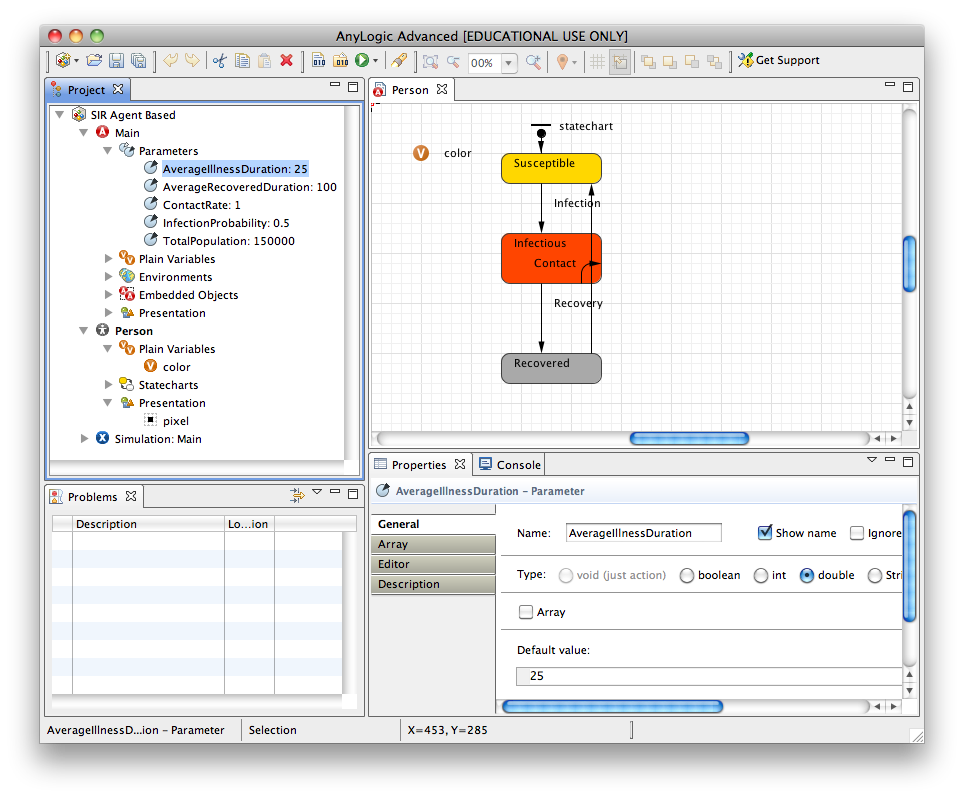
\includegraphics[bb= 0 0 964 798, width=0.5\textwidth]{sir_anylogic.png}
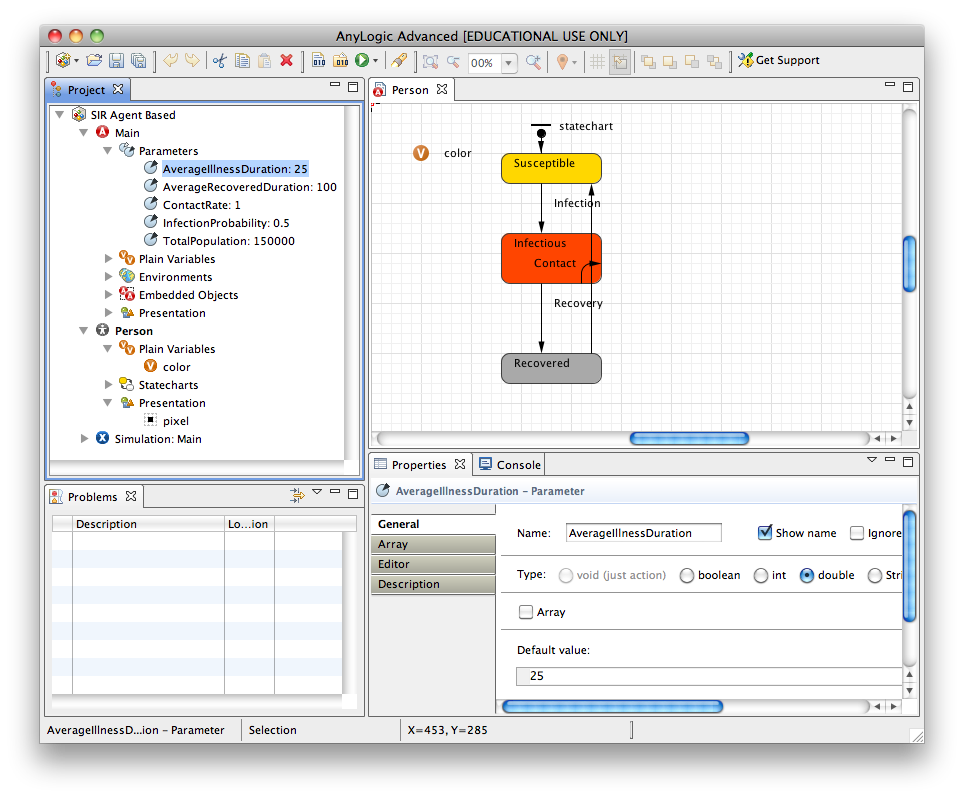
\includegraphics[width=0.5\textwidth]{sir_anylogic.png}
\caption{SIR Model implemented in AnyLogic. Note that, through hiding of information, the user must hunt to find details. On the other hand, if AnyLogic were to show all of the Java code, the result would not be much better. \label{fig:sir_anylogic}}
\end{figure}

%%%%%%%%%%%%%%
%	Section: FRP		%
%%%%%%%%%%%%%%

\section{Functional Reactive Programming}

In this section, we describe the technique of functional programming, its extension to functional reactive programming (FRP), and how we use FRP to represent agent-based health models.

\subsection{Functional Programming}

Functional programming is a programming paradigm in which computer languages define pure functions without mutable state or other computational effects tying them together.  Hence, sequencing of program execution, which is mandated by these effects, is only provided by function calls. These languages are often called declarative languages.  Examples of functional programming languages include Scheme, ML, and Haskell.\footnote{In fairness, Scheme and ML provide some imperative features, but use of these is discouraged.}

Functional programming provides concise and expressive code, often orders of magnitude shorter than imperative languages, and with a structure that often exposes the fundamental algorithm more clearly.  This means that functional programs can be transparent, enabling a computational modeler to debug by inspection.  Essentially, reasoning about functional programs is simpler, involving less of the global execution state, because side effects are reduced and explicit.

However, by avoiding explicit manipulation of the global execution state, it can be difficult to represent a time-varying system in a functional paradigm. In purely-functional programming languages like Haskell, system state is represented as a hidden parameter using monads \cite{essence}. In a non-purely-functional programming language like ML, code must take on an imperative style, compromising elegance and transparency. This makes traditional functional programming poorly suited to agent-based modeling.

\subsection{Functional Reactive Programming}

Functional reactive programming (FRP) endeavors to accommodate sequencing in functional programs by imbuing a language with an intrinsic notion of time \cite{frpcont,yampa}. This allows us to overcome the problem of representing a time-varying system in a functional language. In addition, FRP provides an effective mechanism for visualization of output - indeed, its original purpose was to produce animation \cite{fran}.

%CUT THE FOLLOWING PARAGRAPH AND SUBSEQUENT REFERENCES TO SIGNAL FUNCTIONS IF NECESSARY
%In a functional paradigm, the user works with \emph{functions} and \emph{values}. In FRP, however, these concepts are lifted to \emph{signal functions} and \emph{signals}. A signal is a time-varying value, that is, a function of the type \begin{math} Time \rightarrow \alpha \end{math}, and a signal function is a transformer with the type \begin{math} Signal\ \alpha \rightarrow Signal \  \beta \end{math} \cite{yampa}.\footnote{In this context, $\alpha $ and $\beta$ are type variables} The result is a functional program that executes over time and that can react to different input.

To improve FRP code, Hughes developed the concept of the \emph{arrow} \cite{mon2arr}. Arrows are a generalization of \emph{monads} that are used in functional programming for sequencing. Monads encapsulate computation, forming a list or pipeline of computation that can make a programmer's job easier. An example from Haskell is the IO monad, which is used to transmit the external state of the world as a hidden parameter.

While monads form a pipeline, arrows form a graph; multiple arrows can converge and split. This leads to a natural representation of circuits and dynamic systems. In the case of FRP, arrows are used to implicitly interpret time. Paterson made this approach more transparent with his excellent syntactic sugar - arrows essentially make graphical diagrams in the code, improving readability \cite{PatersonRA:notation}. %See Figure \ref{arrow_syntax} for an example.

%NECESSARY CUT
%example of paterson's arrow syntax
%\begin{figure}[htbp]
%\begin{center}
%\begin{lstlisting}[language=haskell]
%alarm :: SF WInput String 
%alarm = proc inp -> do
%        dMon <- doorMonitor -< inp
%        wMon <- windowMonitor -< inp
%        tMon <- tempMonitor -< inp
%        returnA -< result (dMon 
%                          `lMerge` wMon
%                          `lMerge` tMon)
%\end{lstlisting}
%
%\caption{An example of FRP modeling an alarm system for a building, written in Haskell/Yampa. {\tt doorMonitor}, {\tt windowMonitor}, {\tt tempMonitor}, and {\tt alarm} are all signal functions (SFs), FRP functions with a sense of time. Paterson's syntactic sugar for arrows \cite{PatersonRA:notation} makes the relationships between SFs clear.}
%\label{arrow_syntax}
%\end{center}
%\end{figure}

\subsection{SIR model written with FRP}

We implemented the SIR model in the functional programming language Haskell, using Yale's Yampa \cite{yampa} environment for FRP (see Figure \ref{sir_yampa}). We used the Glasgow Haskell Compiler (GHC) version 6.12.3. For visualization, we used wxFruit, an implementation of Fruit (Functional Reactive User Interface Toolkit) using wxWidget bindings \cite{fruit, wxfruit}.

\begin{table}[!b]
\caption{Source lines of code for model implementations comparing Java code generated by AnyLogic for an executable file and our hand-programmed Haskell/Yampa implementations.}
\label{table:linecounts1}
\begin{center}
\begin{tabular}{| l || c | c |}
\hline
Model & AnyLogic & Haskell/Yampa  \\
\hline
Game of Life & 839 & 70 \\
SIR & 1282 & 70  \\
ESRD/TB & 2222 & 166 \\
\hline
\end{tabular}
\end{center}
\end{table}


Computational models written in Haskell/Yampa were orders of magnitude shorter than their Java counterparts produced by AnyLogic  (see Table \ref{table:linecounts1} for a comparison of source lines of code). Note that while the SIR model is used here as a unifying example, additional models were implemented in Haskell/Yampa and Frabjous but cannot be reported in similar detail due to space limitations. These include Conway's Game of Life, an early example of cellular automata, and ESRD/TB, a model examining the representation and potential outcome of comorbidities of end-stage renal disease and tuberculosis.

% CUT IF NEED BE
%(figure of raw FRP syntax)
\begin{figure}[htbp]
\begin{center}

\begin{lstlisting}[language=haskell]

--states of agents
susceptible :: StateSF
susceptible = dSwitch (constant Sus &&& 
			(arr (/=[]) >>> edge))
		(\_ -> infected)
\end{lstlisting}

\caption{Excerpt from the Haskell/Yampa implementation of the SIR model.}
\label{sir_yampa}
\end{center}
\end{figure}

Many of the models fit on one page of code. However, this conciseness comes at a cost. Though transparent to a programmer familiar with functional reactive programming, much of the syntax is difficult to understand by the layperson. Higher order functions and FRP syntax made the language complicated to those unfamiliar with this programming paradigm (see Figure \ref{sir_yampa} for an example). To overcome this obstacle, we chose to develop an agent-based modeling framework and domain-specific language in Haskell.


%figure for SIR model in Frabjous-generated code
%\begin{figure}[htbp]
\begin{figure}
\begin{center}
\begin{lstlisting}[language=haskell]
-- state definitions for diagram flu
diagram_flu = state_flu_susceptible

state_flu_susceptible = state output
		transitions
     where
        output = State_flu_susceptible
        transitions = transition1
        transition1 = receive "infect" 
        		state_flu_susceptible

\end{lstlisting}
\caption{Excerpt of the Haskell/Yampa code generated by the Frabjous system prototype for the SIR model.}
\label{sir_generated_frp}
\end{center}
\end{figure}

%%%%%%%%%%%%%%%%
%	Section: Frabjous		%
%%%%%%%%%%%%%%%%

\section{Frabjous}

We present an initial specification of Frabjous, our domain-specific language and framework for developing functional reactive agent-based simulation (``FRABjouS''). Frabjous provides a high-level natural language to generate Haskell/Yampa code, which can then be further fine-tuned. Although our system is still a prototype, initial results show promise. The Haskell/Yampa code is concise and human-readable, a rarity for generated code. See Figures \ref{sir_generated_frp} and \ref{sir_frabjous} for examples of generated code and its Frabjous specification.

\subsection{Language Specification}

%Chris, help!
Here we detail the Frabjous language specification. Frabjous describes a labelled transition system. Programmers define a \emph{model}, with an \emph{environment}, a set of \emph{agents}, and a set of \emph{networks} of agents.

%TODO: Reorder, add in examples from the SIR model
A \emph{model} is the top-level system abstraction described by Frabjous. It has a defined name, and encapsulates everything required to run an agent-based simulation.

An \emph{agent} is the bottom-level system abstraction. Each has a unique identifier, as well as a list of associated networks, confounders, diagrams, and populations (described later).

A \emph{diagram} is shorthand for a state-transition diagram. A diagram has a unique identifier, a starting state, and a list of associated states. A \emph{state} is part of a diagram. Each state describes a state of an agent with respect to the distinctions captured in this diagram; for example, in the SIR model, there are three states: Susceptible, Infectious, and Recovered. Every state has unique identifier, a list of messages, a list of variables, a list of transitions to other states in the same diagram, and display information for visualization when the model is in execution. A \emph{transition} is the means by which an agent switches between states. Each transition has a trigger (described below) and a target state.

%figure for SIR model in frabjous
%\begin{figure}[htbp]
\begin{figure}[!b]
\begin{center}
\begin{lstlisting}
discrete model sir

    on startup send "infect" to anyone
	
    network connections of people
    	by vonneumann
	
    diagram flu starting with susceptible
        state susceptible displays yellow
            on receive "infect" switch to
            		infectious
        state infectious displays red
            on timeout 10 switch to recovered
            on rate 1 send "infect" to 
            		neighbour connections
        state recovered displays blue

    agent people with
        flu
        population 100
\end{lstlisting}
\caption{SIR model written in Frabjous.}
\label{sir_frabjous}
\end{center}
\end{figure}


A \emph{message} is the means by which agents communicate to each other. Each message has a \emph{trigger}, an event that will initiate the sending of a message or the transition from one state in a diagram to another. A trigger can be: ``startup'', where the event will trigger when the simulation starts running; ``rate'', a probabilistic method representing a Poisson process where a mean of $x$ triggers will occur per unit of time; ``timeout'', where a trigger will occur after $x$ time units; ``expression'', where a trigger will occur when a boolean expression evaluates to true; ``enter'', where a trigger will occur when an agent transitions to the specified state; and ``leave'', where a trigger will occur when an agent transitions from the specified state.  For example, in the SIR model, an Infectious agent might send a message to another agent to represent contact. If the receiving agent is in the Susceptible state, it will have a probability to switch states to Infectious. An example of a trigger in the SIR model is the infection of patient 0 on startup.

A \emph{target} is a set of agents designated to receive a message. At this point in time, we limit it to: ``anyone'', where one agent at random is selected to receive the message; ``everyone'', where every agent receives the message; ``neighbour'', where an agent's neighbor is selected at random from a specified network; and ``neighbours'', where an agent's entire neighbourhood from a specified network receives the message.  For example, each Infected agent sends a message to {\tt neighbour connections}, where {\tt connections} is the only network defined in the model. We support a number of common neighbourhood definitions (Figure \ref{fig:neighborhoods}).

A \emph{confounder} is a way of combining diagrams, the internal state abstraction for each agent. Each confounder has a list of diagrams to combine, and  a list of messages that provide greater control over ways these diagrams interact. In this way, health modelers can study the interaction between different diseases. We defer a discussion of this to Section \ref{sec:confound}.

%ESRD/TB state diagram
%\begin{figure}[h]
%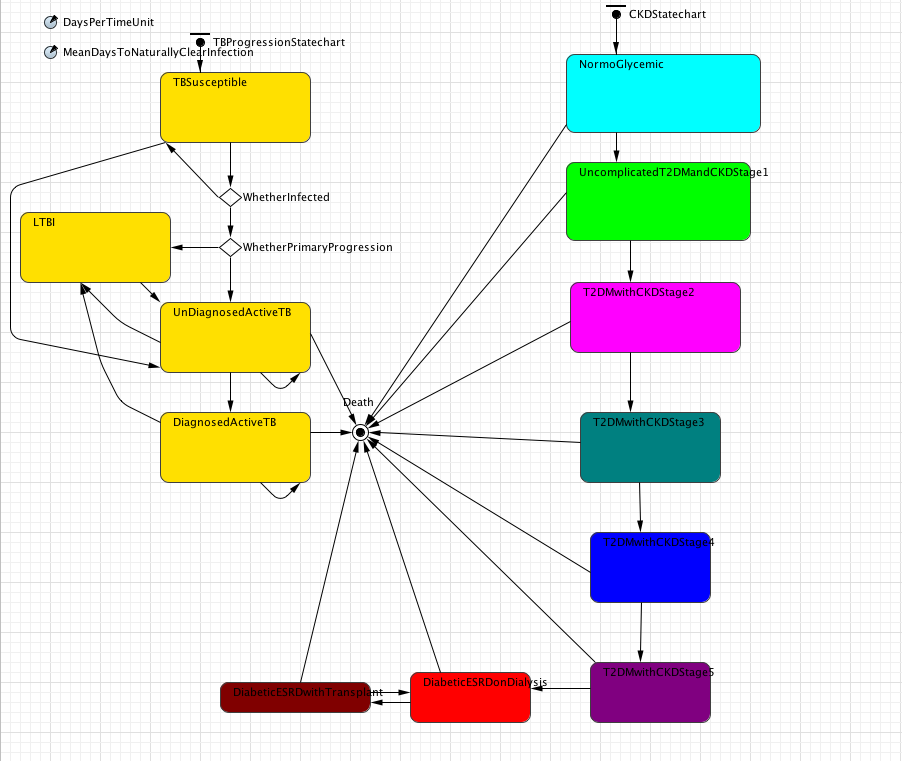
\includegraphics[width=0.5\textwidth]{esrd_tb_state.png}
%\caption{The state diagram for the ESRD/TB model in AnyLogic. This model has two disease that influence each other - the rate of progression in the ESRD model on the right depends on the current state in the TB model on the left. This is not immediately clear from the structure.}
%\label{fig:esrd_tb_state}
%\end{figure}

A \emph{network} is an arrangement of agents describing how they are connected to each other. Each network has a unique identifier, the identifier of a type of agent, and a \emph{structure}, a defined method for creating \emph{neighborhoods} in a network. Network structure depends on the model's \emph{environment}, which is either discrete or continuous.


%Example of neighbourhoods
\begin{figure}[h]
%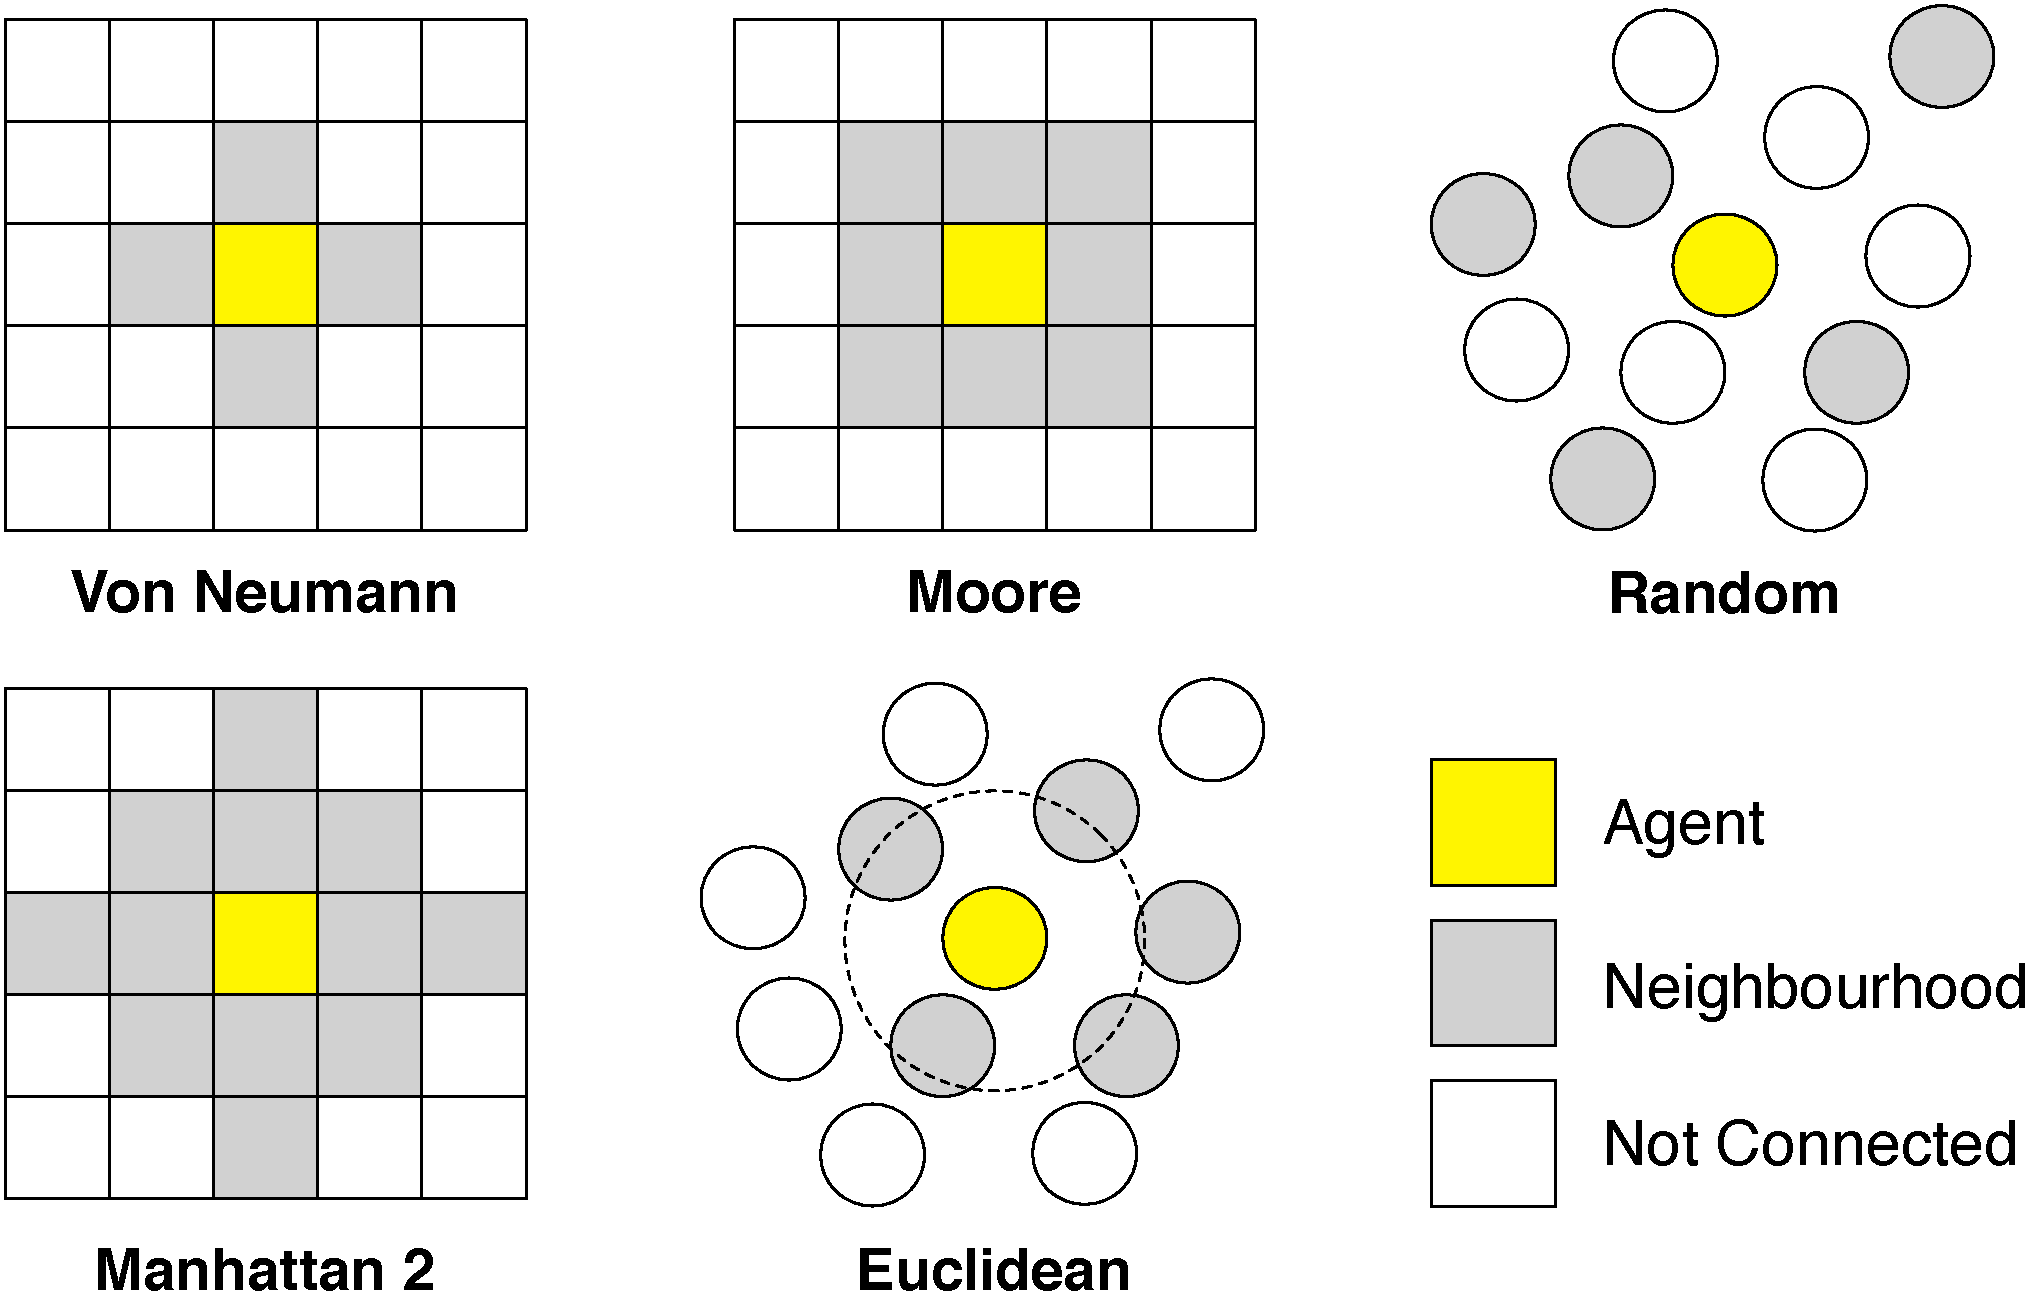
\includegraphics[bb= 0 0 1016 653, width=0.48\textwidth]{neighbourhoods.pdf}
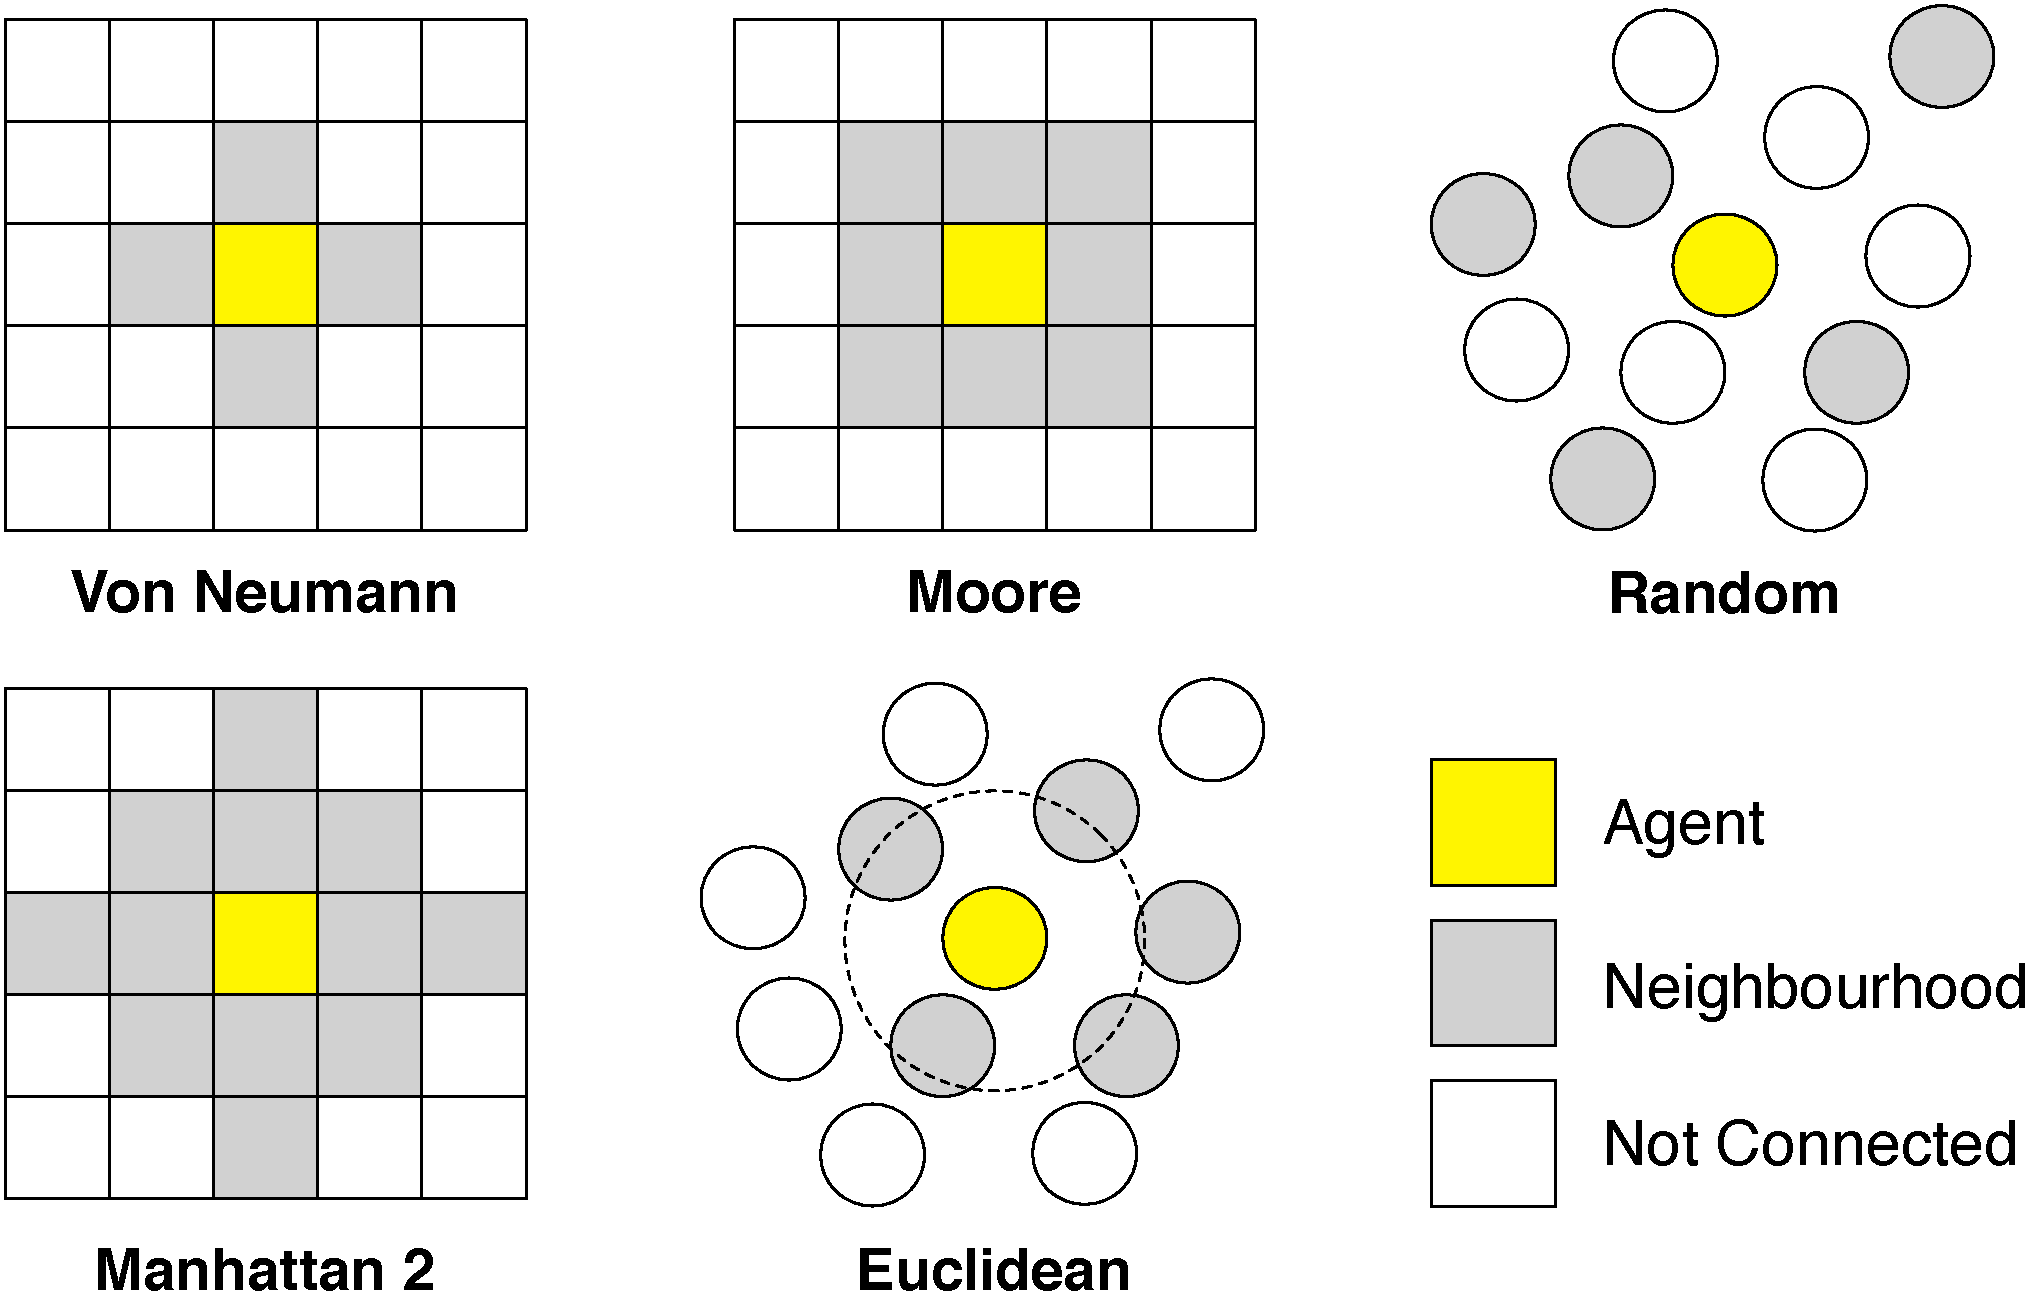
\includegraphics[width=0.48\textwidth]{neighbourhoods.pdf}
\caption{Examples of different types of neighbourhoods. Moore, Von Neumann, and Manhattan neighbourhoods are only available in a discrete environment where agents form a grid. Euclidean and Random neighbourhoods are only available in a continuous environment, where agents are distributed randomly in 2D space.}
\label{fig:neighborhoods}
\end{figure}


\subsection{System Description}

The Frabjous system has two components: a compiler, which generates Haskell/Yampa code from a Frabjous model specification, and a Haskell/Yampa library intended to make generated code more readable. We hope to use the Frabjous specification as a way to rapidly develop initial models, and then provide the full programming environment of Haskell/Yampa to tweak or further improve more sophisticated models. Our goal is to have modelers develop at both levels, and be able to see the entire model at a glance from either representation.

% See Figure \ref{fig:frabjous_system_diagram} for a high-level overview of the system.

%NECESSARY CUT
%\begin{figure}[h]
%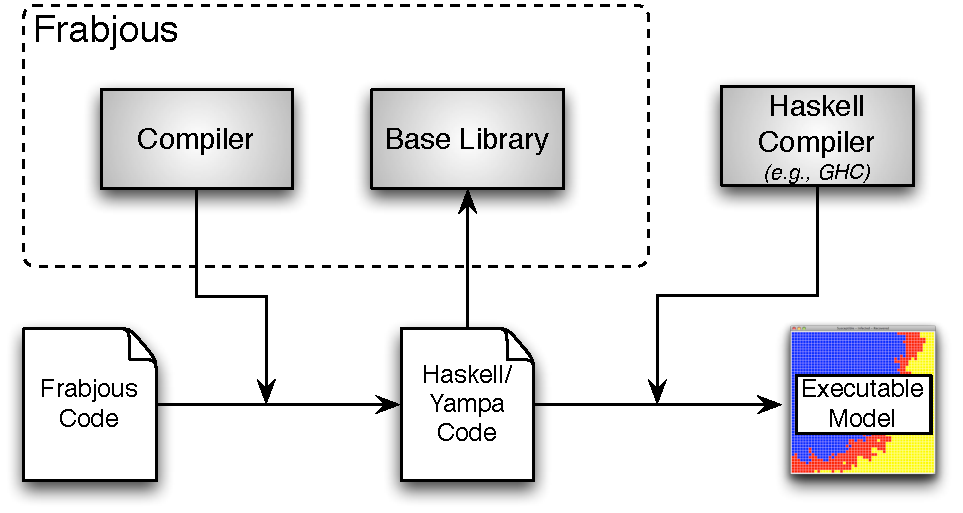
\includegraphics[width=0.48\textwidth]{Frabjous_HighLevelSystem.pdf}
%\caption{A high-level overview of the Frabjous system. \label{fig:frabjous_system_diagram}}
%\end{figure}

The Frabjous compiler was developed in Haskell/Yampa using the Parsec library \cite{parsec}. The system is partially implemented; the parsing module and rudimentary type-checking are complete and the code generator is partially implemented. The Frabjous library is still under development. The Glasgow Haskell Compiler (GHC) will be used to compile generated code into a binary executable.

\subsection{Language Features}

%TODO!
Our partial implementation shows promising results in human-readable generated code. In addition, both representations are extremely concise (see Table \ref{table:linecounts1}). Hand-crafted Haskell/Yampa code is approximately four times shorter than the Java code generated by AnyLogic. Frabjous-generated Haskell/Yampa code length is expected to be similar to that of our hand-crafted examples.


%TODO!
The higher-level character of the specification helps in maintaining modeler reasoning at the domain level, which is important in creating, extending, debugging, and seeking to understand a model. Through Frabjous, modelers can think in terms of the domain rather than at the level of a programming language.

\subsection{The Confound Statement}
\label{sec:confound}
One particularly exciting feature of Frabjous is the \emph{confound} statement. This statement allows two different models to be combined and interact in a defined way. We hope to provide modelers with the ability to confound agent-based models in a fashion similar to that used by functional programmers to compose functions. The combinatorial explosion of combining different simulations (for example, simulating two or more diseases interacting within a single agent) is poorly handled in aggregate simulation models \cite{osgood_comorbidities}. While agent-based tools can avoid this combinatorial explosion, modular specification of comorbidities  is not supported in a modular fashion in existing agent-based simulation tools. Comorbidities are common, and the opportunity to capture their dynamics in a clean fashion is a significant motivator for using agent-based simulation. Through the confound statement we hope to provide increased manageability of large model sets and better support collaboration between modelers.


%%%%%%%%%%%%%%%%
%	Section: Summary		%
%%%%%%%%%%%%%%%%

\section{Summary}

We have demonstrated a need for more transparent and efficient tools (in terms of both computational resources and human skills) in the domain of agent-based health simulation. We have provided a case for using functional reactive programming to meet this need. Initial exploration revealed that this approach yields concise and transparent code for expert programmers, but a language barrier for less-experienced programmers. The development of a domain-specific language and domain library (Frabjous) compensates for these problems and presents a step towards a viable solution.

%%%%%%%%%%%%%%%%
%	Section: Future Work	%
%%%%%%%%%%%%%%%%

\section{Future Work}

We plan to complete the implementation of the Frabjous system by finishing the code generation and base library modules. Iterative design and evaluation with additional health modelers will provide a deeper understanding of how to effectively develop a tool that is transparent, effective, and easy for modelers to use.

To address this need, there are planned improvements to evaluate the computational efficiency by parallelization. We plan to use CUDA to compute each agents' actions and interactions in parallel at each time step. Preliminary investigation suggests that this will be a simple conversion \cite{dphaskell}, but one that could offer important incentives for using the Frabjous framework.

%ACKNOWLEDGEMENTS
\section{Acknowledgements}
%{\em Acknowledgements removed for anonymous review}
This work was funded in part by a Natural Science and Engineering Research Council of Canada (NSERC) Undergraduate Student Research Award (USRA), an NSERC CGS M scholarship, and the NSERC Discovery Grants program.

%%%%%%%%%%%
%BIBLIOGRAPHY   %
%%%%%%%%%%%
%\nocite{*}
%\bibliographystyle{plainnat}
\bibliographystyle{abbrv}
\setlength{\bibsep}{0.5ex}
\bibliography{refs}


%%%%%%%%%%%
%	APPENDIX 	%
%%%%%%%%%%%

%\appendix
%\section{Appendix}

%source code for sir.hs
%\lstinputlisting{src/sir.hs}


\end{document}
\endinput
